\section{Stand der Technik}
\subsection{Einsatz und Aufbau von Kompressoren}
Die Aufgabe von Kompressoren ist es Gase zu komprimieren.
In diesem Fall nimmt die Dichte der Gase zu, gleichzeitig wird das
Volumen verkleinert.
Dar"uber hinaus steigen die Temperatur und der Druck durch die resultierte
Kraft, die gebraucht wird, um die Gase entgegen ihres nat"urlichen
Verhaltens zu verdichten. [2] 
Es gibt zwei Arten von Kompressoren, einen Kolbenkompressor
und einen Schrauben-Kompressor. 
In der Arbeit wird ein Kolbenkompressor benutzt,
auf diese Bauweise n"aher eingegangen.Den Aufbau eines typischen
Kolbenkomprerssor sehen Sie in Abbildung~\ref{fig:komp1}.

\begin{figure}[!htb]
\begin{center}
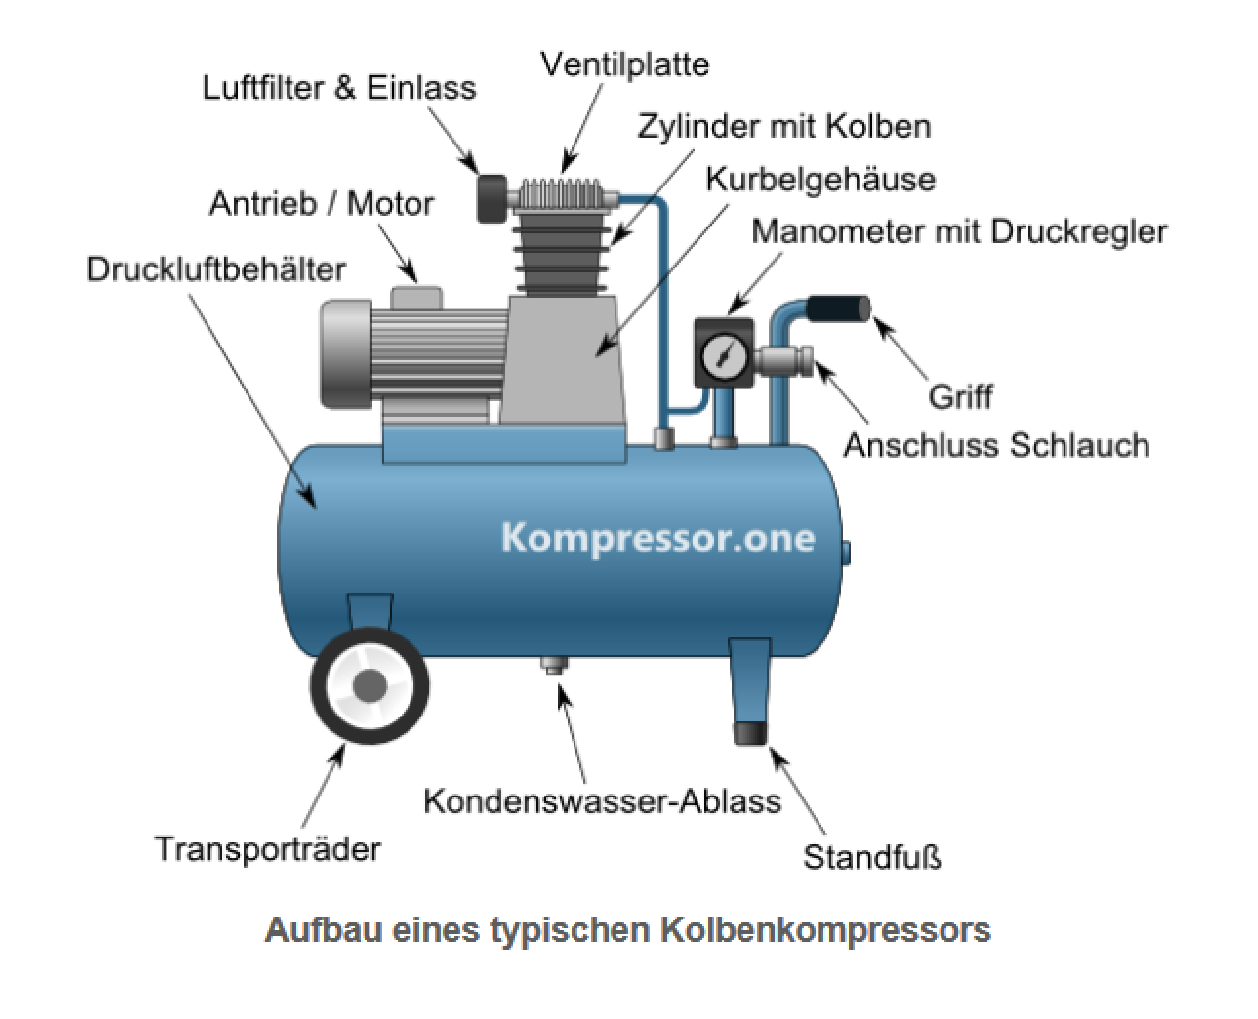
\includegraphics[height=7cm]{bilder/Kompressor.eps}
\end{center}
\caption{Aufbau eines typischen Kompressors}\label{fig:komp1}
\end{figure}

Sobald der Kolbenverdichter in Betrieb ist,
wird sich der Kolben,
der mit einer Dichtung zur Zylinderwand hin abgedichtet ist, 
hin und her bewegen. 
Wenn sich der Kolben zurückzieht, 
wird Luft durch das Einlassventil wie gezeigt in Abbildung~\ref{fig:komp2} angesogen 
und wenn sich der Kolben wieder vorschiebt, 
schlie"st sich dieses Ventil  
 und die Luft wird zusammengedrückt 
und wiederum wie gezeigt in Abbildung~\ref{fig:komp3} durch das Auslassventil abgegeben.


\begin{figure}[!htb]
\begin{center}
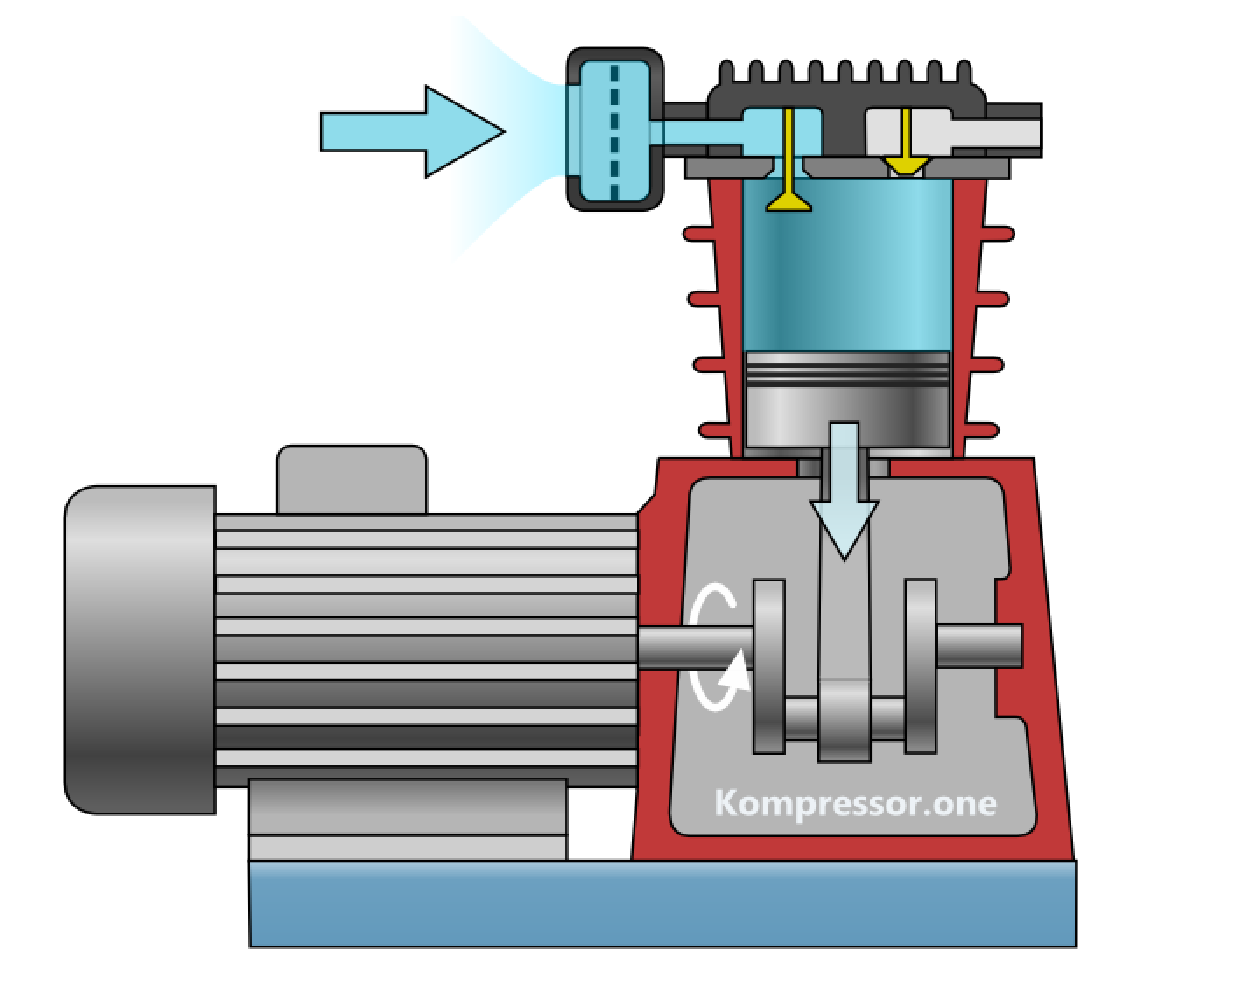
\includegraphics[height=7cm]{bilder/Kom2.eps}
\end{center}
\caption{Ansaugen}\label{fig:komp2}
\end{figure}

\begin{figure}[!htb]
\begin{center}
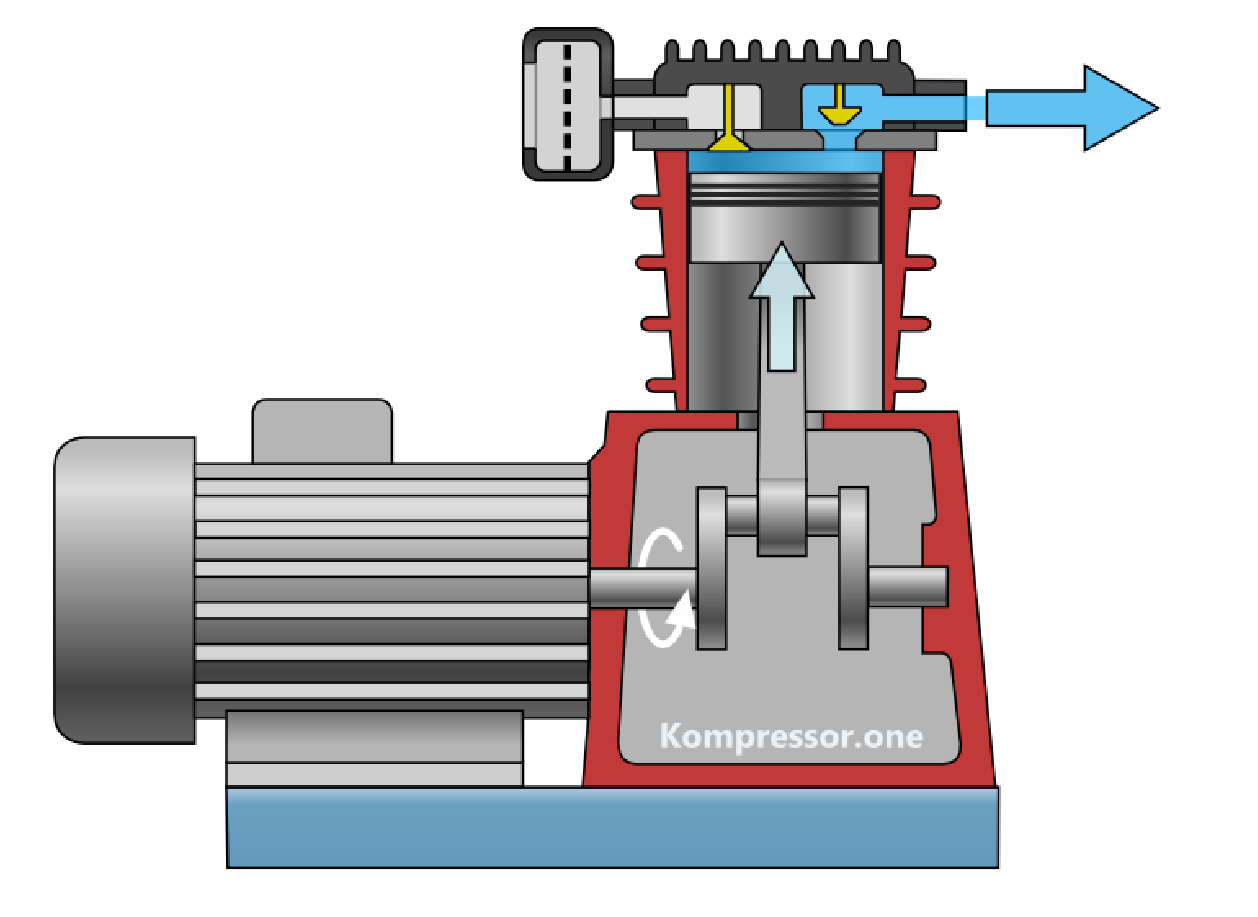
\includegraphics[height=7cm]{bilder/kom3.eps}
\end{center}
\caption{Verdichten}\label{fig:komp3}
\end{figure}

Der Aufbau und das Prinzip des Kolbenkompressors "ahnelt 
sehr einer handels"ublichen Luftpumpe. 
Formen und Gef"a"se, wie z.B. Tanks die unter Druck stehende Gase oder 
Flüssigkeiten aufnehmen sollen, 
k"onnen ebenso auf die gleiche Weise befüllt werden. 
Selbst bei der Produktion von PET-Flaschen wird die Funktionsweise 
von Kolbenverdichtern angewendet. 
Kolbenverdichter werden in Automotoren eingesetzt,
 um die Leistung zu erh"ohen,
 indem sie mehr Luft in die Brennkammern bef"ordern. 
 Als weiteres wichtiges Merkmal ist zu benennen, 
 dass die Verdichter nicht f"ur den konstanten Gebrauch vorgesehen sind 
 und nur zeitweise Arts gem"a"s zum Einsatz kommen.[2] 
 
 \subsection{Wichtige pysikalische Kenngr"o"sen des Kompressors}
 
 Wichtige Parameter des Kompressors sind die Volumenf"ordermenge des 
 F"ordermediums pro Zeiteinheit und der Betriebsdruck, der durch den 
 eventuellen "uberh"ohten Druck der Druckluft bezeichnet wird. Ein weiterer 
 wichtiger Parameter ist das Druckverh"altnis, das sich aus dem Verh"altnis 
 zwischen Enddruck und Saugdruck ergibt. Der Durchfluss zeigt das Verh"altnis
  zwischen dem Volumenstrom der gef"orderten Druckluft und 
  dem theoretisch m"oglichen Volumenstrom[37].
  
 Die Ansaugleistung ist die Luftmenge, die das Ger"at ben"otigt, 
  um es zu verdichten und in Druckluft umzuwandeln. Der Wert wird in 
  Liter pro Minute (L/min) angegeben. Die Ansaugleistung eines 
  Kolbenkompressors ist immer höher als die Ausgangsleistung, was viel wichtiger ist.
   Die Saugleistung ist daher nicht ideal als Kenngröße und
    nur bedingt nutzbar.\newline
    
    Die Gr"o"se des Kessels gibt das Volumen des Druckluftbeh"alters an. 
    Abh"angig von den Anforderungen und der Nutzung kann das Kesselvolumen 
    ein relevanter Kontrollwert f"ur Kompressoren sein. Dieser Kenngr"o"senwert 
    des Kompressors gibt das Bef"ullungsvolumen des Druckluftbeh"alters an.
    Je gr"Oßer die Kesselgr"Oße, desto gr"Oßer die Druckluftversorgung und umso mehr 
    wird der Kompressor eingespart, da er nicht  so h"aufig starten muss.
     Erst wenn ein Mindestdruck im Tank erreicht ist, startet der Motor wieder.
     Die Gr"Oße des Kessels wird in Liter angezeigt.\newline
     
     Der maximale Druck eines Kompressors repr"asentiert den 
     h"ochstm"oglichen Grad der Luftverdichtung, der mit dem 
     entsprechenden Drucklufterzeuger erreicht werden kann. 
     Entgegen den Erwartungen ist dieser Vergleichswert von
      Kompressoren in vielen F"allen nicht sehr wichtig. 
      Tats"achlich ist ein au"sergew"ohnlich hoher Luftdruck nur 
      bei sehr wenigen Arbeiten erforderlich. In den meisten 
      F"allen gen"ugt ein durchschnittlicher Druck, so dass dieser 
      Vergleichswert nur im Einzelfall f"ur eine Kaufentscheidung 
      entscheidend sein sollte.
Der Druck wird ebenfalls in bar gemessen[39].
    
  
  
  
 

\subsection{Der Encoder}
Der Drehgeber wird auch Wellencode genannt und ist wie ein Encoder,
 Winkelmesser oder ein Ger"at, 
 das auf der Basis einer mechanischen Bewegung 
 bzw. einer Rotation arbeitet
  und sie in ein elektrisches Ausgangssignal umwandelt. 
  Es gibt zwei Haupttypen: Absolutwertgeber, 
  der die aktuelle Position der Welle angibt, 
  deshalb wird er als Winkel-Messumformer dienen und Inkrementalgeber, 
  der die Daten liefert, um die Welle zu bewegen. 
  Au"serdem werden andere Daten wie Drehzahl, 
  Position und Entfernung verarbeitet. 
  Verschiedene Sensortechnologien k"onnen vom Encoder benutzt werden. 
Die am meisten verwendete Bauart ist die optischen Encoder.
  Eine Lichtquelle leuchtet bei einem optischen Encoder, 
  wenn die Scheibe dreht. 
  Sie ist markiert, dass das Licht scheint oder blockiert wird. 
  Der Sensor nimmt das Scheinen des Lichtes 
  und bildet einen angemessenen Impuls[3].
  Den Aufbau und die Signalausgabe bei Rotation sehen Sie 
  in Abbildung~\ref{fig:Encoder} 
\begin{figure}[!htb]
\begin{center}
\includegraphics[height=7cm]{bilder/Encoder.eps}
\end{center}
\caption{Optischer Encoder mit optischen Sensor und einer optischen Scheibe zur Winkelmessung[3]}\label{fig:Encoder}

\end{figure}


Die rotierende Scheibe hat maximal 3 Spuren.
Eine oder zwei "au"sere Spuren, 
die in (n) Intervalle gleichen Winkeln abwechselnd undurchsichtig 
und transparent unterteilt sind.  
 Bei einer
vollen Rotation des Encoders wird 
der Lichtstrahl (n) mal unterbrochen und liefert (n) diskrete Signale. 
Der Verschub aus 90$^\circ$ der elektrischen Signale A und B erlaubt es, 
die Drehrichtung zu bestimmen:  
 \newline
In eine Richtung w"ahrend der aufsteigenden Front des Signals A, 
Signal B ist Null. 
Auf der anderen Richtung w"ahrend der Menge Front des Signals A ist 
das Signal B eins.
Die innere Spur (Z: Top Null) hat ein transparentes Fenster und 
liefert pro Runde ein einziges Signal. 
Dieses Z-Signal mit einer Dauer von 90$^\circ$ elektrisch 
bestimmt eine Referenzposition und erm"oglicht den Reset bei jedem Zug. 

Die Counting/Decounting von Impulsen durch die Verarbeitungseinheit
erm"oglicht es,  die Position zu definieren[6].


Vor 30 Jahren wurden Resolver in den meisten Anwendungsgebieten 
statt optische Encodern benutzt. Die Situation sieht heute anders aus.
 Weil die Encoder eine wichtige Rolle spielen und 
 von verschiedene Herstellern hergestellt werden. 
 Optische Encoder verlangen keine getrennte Elektronik. 
 Das aufnehmende Steuerungssystem nutzt die Ausgabedaten, 
 damit sie einfach und spezifiziert eingebaut werden. 
 Der Nachteil ist, 
 dass sie nicht f"ur komplizierte Anwendung wie Schwingungen 
 und  H"ohere Temperaturen geeignet sind und
 es  keine Alarmierung vor einem Defekt gibt[3].

\subsection{Schaltung des Encoders}
\begin{figure}[!htb]
\begin{center}
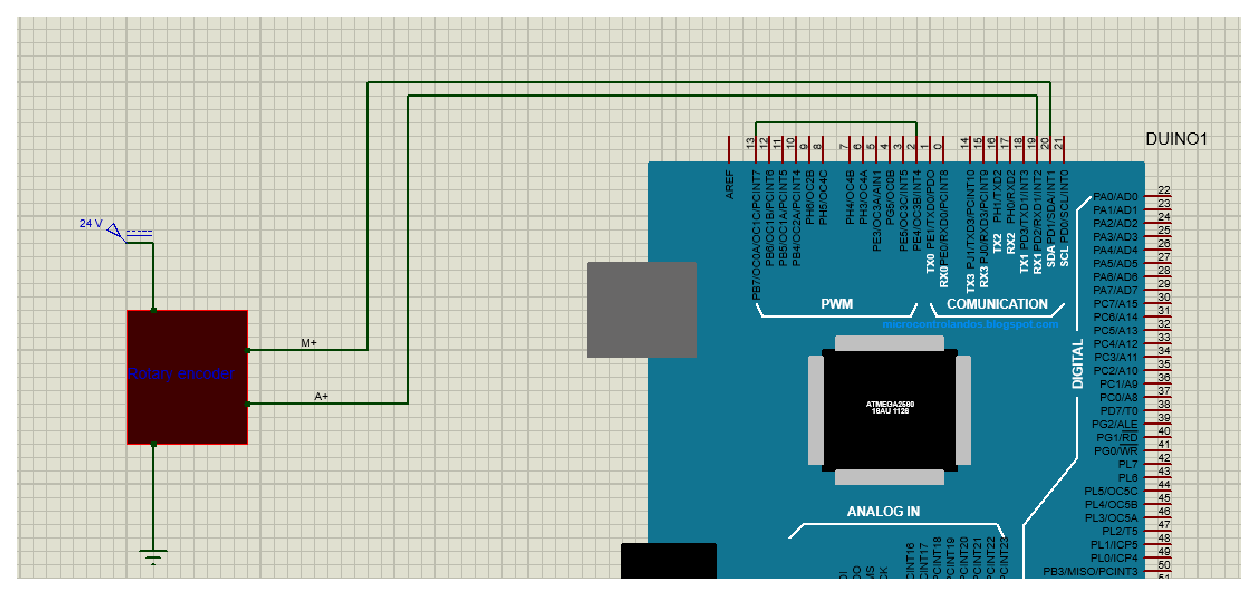
\includegraphics[height=9cm]{bilder/Rot.eps}
\end{center}
\caption{Schaltung des Encoders}
\end{figure}

\subsection{Drucksensor}
\begin{figure}[!htb]
\begin{center}
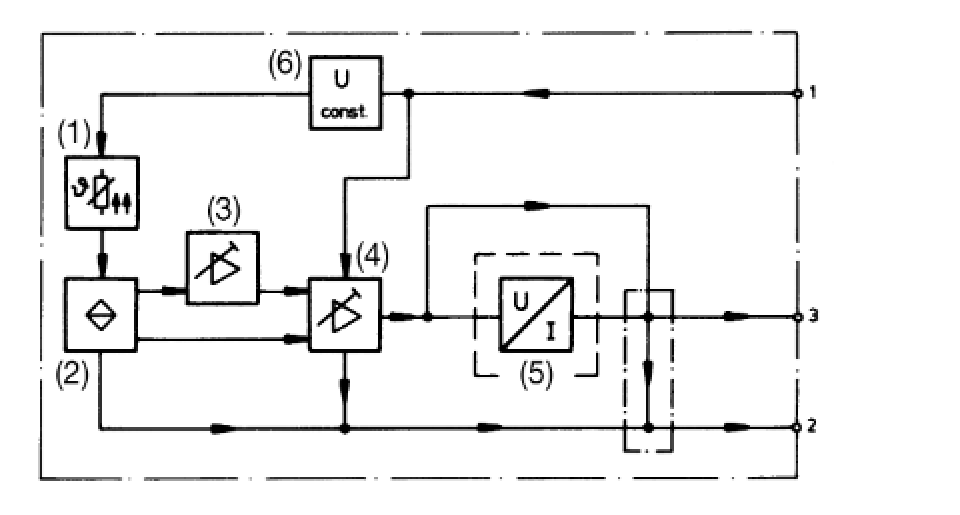
\includegraphics[height=7cm]{bilder/Blo.eps}
\end{center}
\caption{Blockschaltbild[4]}\label{fig:Blo}
\end{figure}


Der Drucksensor funktoiniert indem die druckbelastete Trennmembran 
auf den piezoresistieven Druckmessumformers dr"uckt.

Die  Trennmembran f"uhrt den Druck durch den systematischen Aufbau eines
solchen Drucksensors in Abbildung~\ref{fig:Blo}  
eine Fl"u"ssigkeit der Siliziummembrane mit Widersrandme"ssbr"ucke(2),
die nach dem piezoresistiven Effekt arbeitet und 
"uber eine Temperaturkompensation(1) an eine Konstantspannugsquelle (6)
angeschlo"ssen ist.
Das Ausgang"ssignal der Widerstandsme"ssbr"ucke ist mit
einem Differenzverst"arker mit hohem Eingangswiderstand (4) verst"arkt.
Die Me"ssspanne wird mit Hilfe eines Me"ssspannentrimmers eingestellt.
Eine Nullpunktkorrektur wird vom Verst"arker (3) mit einstellbarer 
Verst"arkung eingestellt. Der Ausgangssignal ist  
 von 0 bis 20 mA .Durch der U/I-Wandler(5) wird 
 das Ausgangssignal in einen angeeigneten Strom umgewandelt. [4]
 
 \begin{figure}[!htb]
\begin{center}
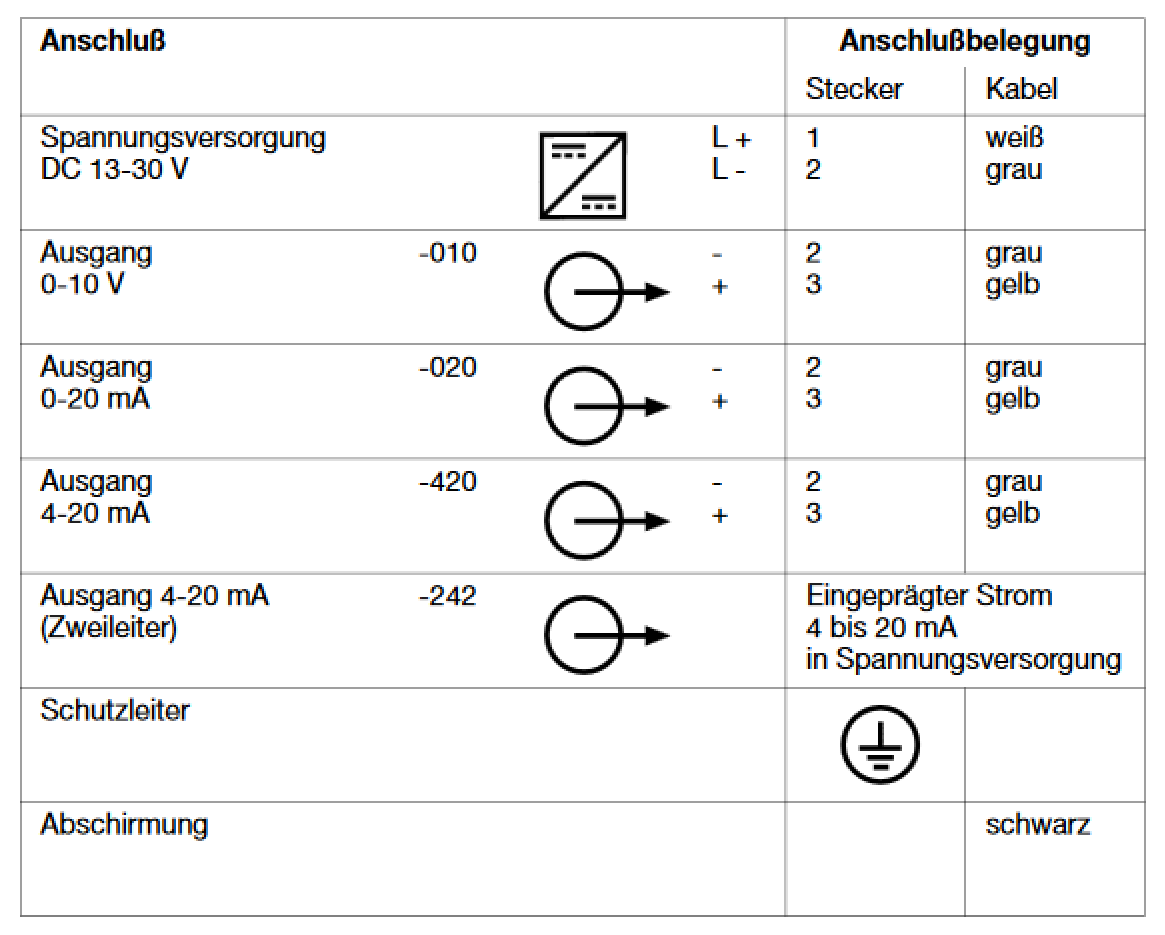
\includegraphics[height=7cm]{bilder/Anschluss.eps}
\end{center}
\caption{Anschlu"ssbelegung[4]}
\end{figure}

Der Referenzdruck ist entweder absolut, 
relativ oder versiegelt. 
  
 Im ge"offneten Raum entspricht der Absolutdruck dem Atmossp"ahrendruck.


Die Differenz zwischen dem absoluten Druck und dem atmosph"arischen ist 
der relative Druck .Der Druck im Beh"alter ist ein bekannter Druck .
Es ist wichtig ,den genauen Referenzdruck zu w"ahlen ,
weil es mehr oder weniger  Fehler eintreten k"onnte[8].

\subsection{PT100 Temperaturf"uhler}

Die maximale Temperatur des Eingriffs und 
die Umgebungstemperatur m"ussen   ber"ucksichtigt werden. 
Die meisten elektronischen Sender des Sensors werden  
nicht richtig funktionieren, 
wenn die Temperatur "uber  107$^\circ$C(225$^\circ$F) l"auft. 
Deswegen ist der Einsatz des entsprechenden Montagezubeh"ors
 zum Beispiel ausreichende L"angen der Impuls, 
 Spulen und so weiter  erforderlich, 
 um  die Sendezelle akzeptable Temperatur der Fl"ussigkeit zu 
 reduzieren. 
 Die Exposition der Elektronik mit Halbleiter der 
 Umgebungstemperaturen hat den Effekt der 
 Besch"adigung von Komponenten. 
 Die meisten elektronischen Bauteile
  k"onnen  nicht  "uber eine Temperatur  
 von 93$^\circ$C(200$^\circ$F)funktionieren  und es gibt eine große Anzahl 
 von Komponenten mit einer maximalen Betriebstemperatur 
 von 85$^\circ$C (185$^\circ$F). 
 Die hohen Temperaturen f"uhren tendenziell
 zu sinkenden elektronischen Energieeffizienz. 
 Auch hier wird empfohlen, 
 die bestm"ogliche K"uhlung des elektronischen Moduls zu gew"ahrleisten.
 Vorstellbar ist auch ein System des Winterschutzes 
 der Elektronik entweder  
 durch Heizdampf, elektrisch oder mittels Thermostat[7].
 
Pt100 ist ein Platin-Widerstand mit einem Nennwiderstand 
von 100$\Omega$ bei einer Temperatur von 0$^\circ$C ,
der in IEC 751 (EN 60751) definiert ist .
Auf Englisch nennt man ihn Resistance Temperature Detector. 
Seit lang werden die Pt100 wie gezeit in Abbildung ~\ref{fig:pt100} in industriellen Unternehmen und 
im Labor benutzt. 
Es gibt auch  andere Pt500 und Pt1000.

\begin{figure}[!htb]
\begin{center}
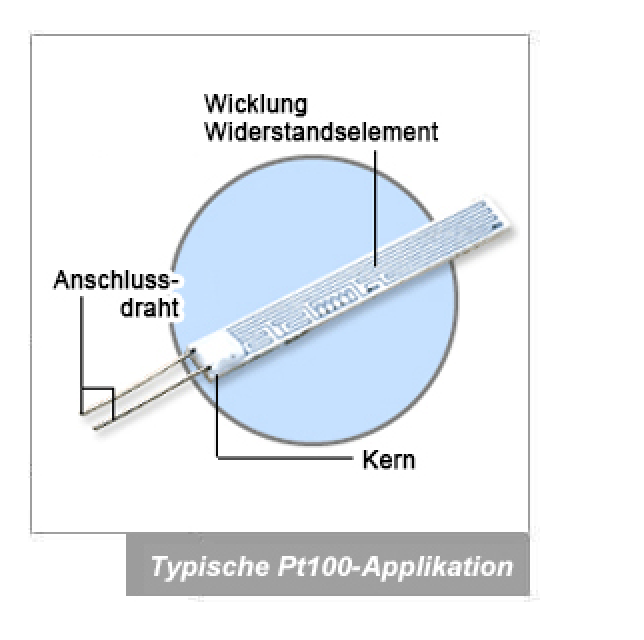
\includegraphics[height=5cm]{bilder/pt100.eps}
\end{center}
\caption{Typische Pt100-Applikation[5]}\label{fig:pt100}
\end{figure}
 
 Pt100 sind stark und nicht empfindlich gegen elektrische St"orungen,
 deshalb sind sie f"ur viele Benutzungen geeignet.
 Außerdem k"onnen die auch in der N"ahe von andere Ger"aten, 
 Motoren und Generatoren gebaut werden, die hohe Spannungen liefern.
 Pt100 haben noch andere Vorteile, die k"onnen große 
 Temperaturbereich von -200$^\circ$C bis 850$^\circ$C messen und lineare sind.
 Außerdem haben die gute Genauigkeit und Austauchbarkeit  
 sowie hohe Stabilit"at f"ur Langzeit[5]. 
 
 \subsection{Bauarten der Pt100}
 
 Alle pt100 sind mit Platin-D"unnschichttechnik produziert, 
 die auf mikrostrukturierten Schichtverbindungen aus Metall, 
 Glas und Keramik basiert. Dar"uber hinaus enthalten die Pt100  
 Sensorelemente aus einer d"unnen Platin-Drahtwicklung, 
 die mit einem Keramik oder Glask"orper verbunden sind.
 Das Element vom Widerstand steckt "ofter in einem Mantelf"uhrer 
 oder einem gleichen sch"utzenden Geh"ause. Auch unter komplizierte 
 Industriebedingungen sind die Pt100 Sensoren stark,
 pr"azise und stabil f"ur lange Zeit.Den Aufbau eines typischen Platin-D"unnschichttechnik
 sehen Sie in Abbildung~\ref{fig:pla}[5].

 
 \begin{figure}[!htb]
\begin{center}
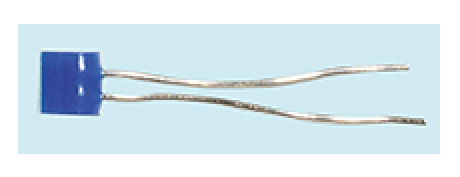
\includegraphics[height=3cm]{bilder/pla.eps}
\end{center}
\caption{Platin-D"unnschichttechnik[5]}\label{fig:pla}
\end{figure}
 
 Um die Widerstandselements zu herstellen, 
 ist es notwendig ein Platin-Material zu nutzen, 
 dessen Widerstand bei unterschiedlichen Temperaturen anerkannt 
 und beschrieben ist. Es gibt eine Widerstands"anderung bei 
 der Temperatur"anderung .Damit die Temperatur aus dem 
 Widerstand abgelesen werden kann,
Eine wichtige Bauart f"ur Pt100  ist der Drahtgewickelte-Widerstand 
wie gezeigt in Abbildung~\ref{fig:dra}. 
Gleichzeitig gibt es zwei Ausstattung  ein mit der Wicklung in einem 
Keramik oder Glasr"ohrchen ,die am meisten verbreitet ist und 
mit der Wicklung außen auf einen Keramik oder Glaskern ,
die mit einer weiteren Glas- oder Keramikschicht  
die f"ur spezielle Umwelteinfl"usse ausgelegt ist[5].

\begin{figure}[!htb]
\begin{center}
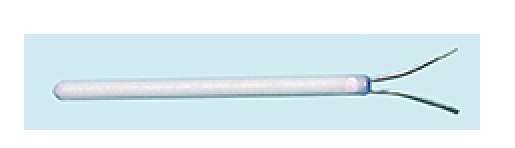
\includegraphics[height=3cm]{bilder/dra.eps}
\end{center}
\caption{Drahtwickelte-Widerstand[5]}\label{fig:dra}
\end{figure}

\subsection{Schaltung der TP100}
\begin{figure}[!htb]
\begin{center}
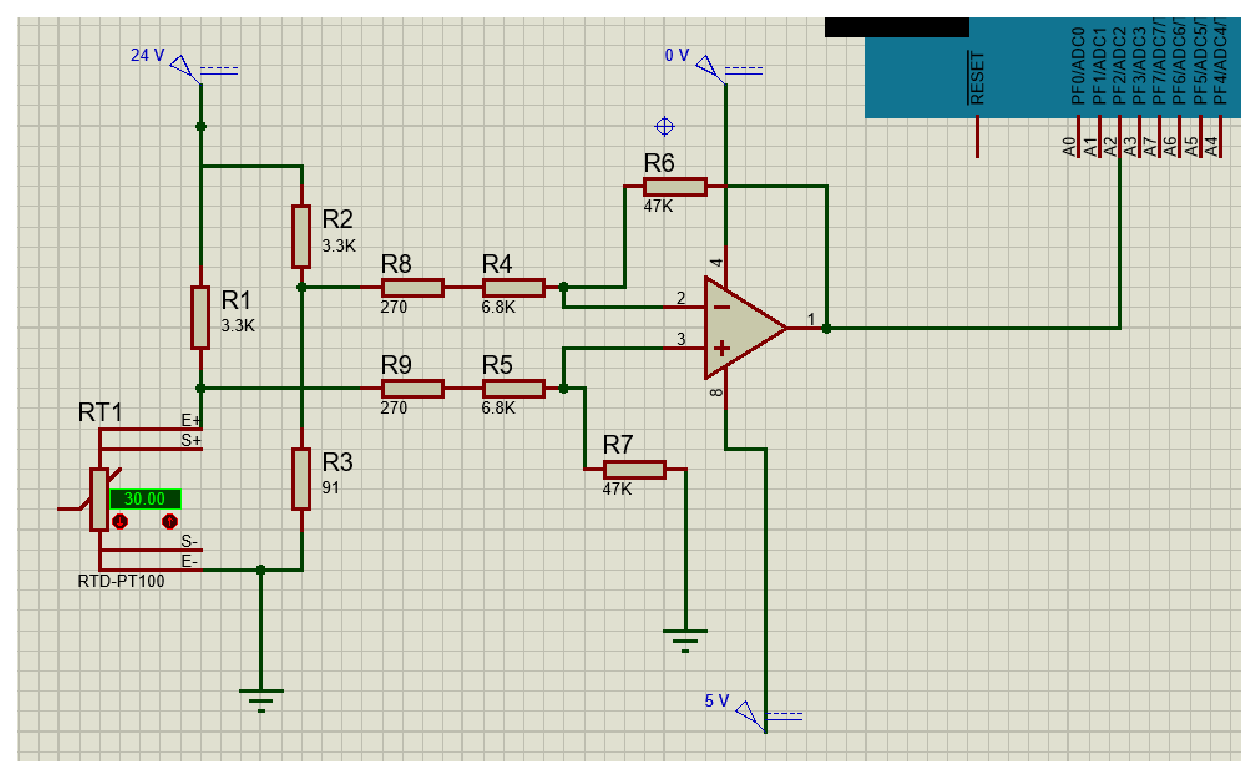
\includegraphics[height=8cm]{bilder/im.eps}
\end{center}
\caption{Schema der Aufbau von TP100}
\end{figure}

\subsection{Dehnmessstreifen}
Ein DMS ist ein Sensor, 
bei dem der Widerstandswert mit der Ausdehnung variiert.
 Die Widerstands"anderung ist auf die minimale Ver"anderung 
 der Linienstruktur im Falle einer Verformung zur"uckzuf"uhren. 
 Wenn der Leiter in L"angsrichtung gestreckt wird, 
 ist die Leiterstruktur d"unner und l"anger, 
 was zu einer gr"oßeren Festigkeit f"uhrt. 
 Diese kleinste Widerstands"anderung gilt als Messwert. 
 Um die Sensibilit"at der DMS zu erh"ohen, 
 sind sie in M"aanderform, was den Leiter als Ganzes verl"angert. 
 In der elektronischen Schaltungstechnik werden Br"uckenschaltungen eingesetzt,
  wenn es darum geht, 
  minimale Schwankungen von Spannung, 
  Strom oder Widerstand zu erkennen. 
  Dies gilt auch f"ur Dehnungsmessstreifen. Um relativ kleine 
  Widerstands"anderungen zu erkennen, werden Dehnungsmessstreifen 
  in Br"uckenschaltungen wie der Wheatstone-Br"ucke angeschlossen und 
  Spannungsdifferenzen in nachgeschalteten Differenzverst"arkern verst"arkt[31].
  
\subsection{DY-Dehnungsmessstreifen}
Die DY-DMS haben zwei parallel angeordnete Messgitter. 
Die typische Anwendung dieser DMS ist die Messung an Biegestangen.Der Aufbau 
eine DY-DMS wird in Abbildung~\ref{fig:DY}gezeigt[26]. 


\begin{figure}[!htb]
\begin{center}
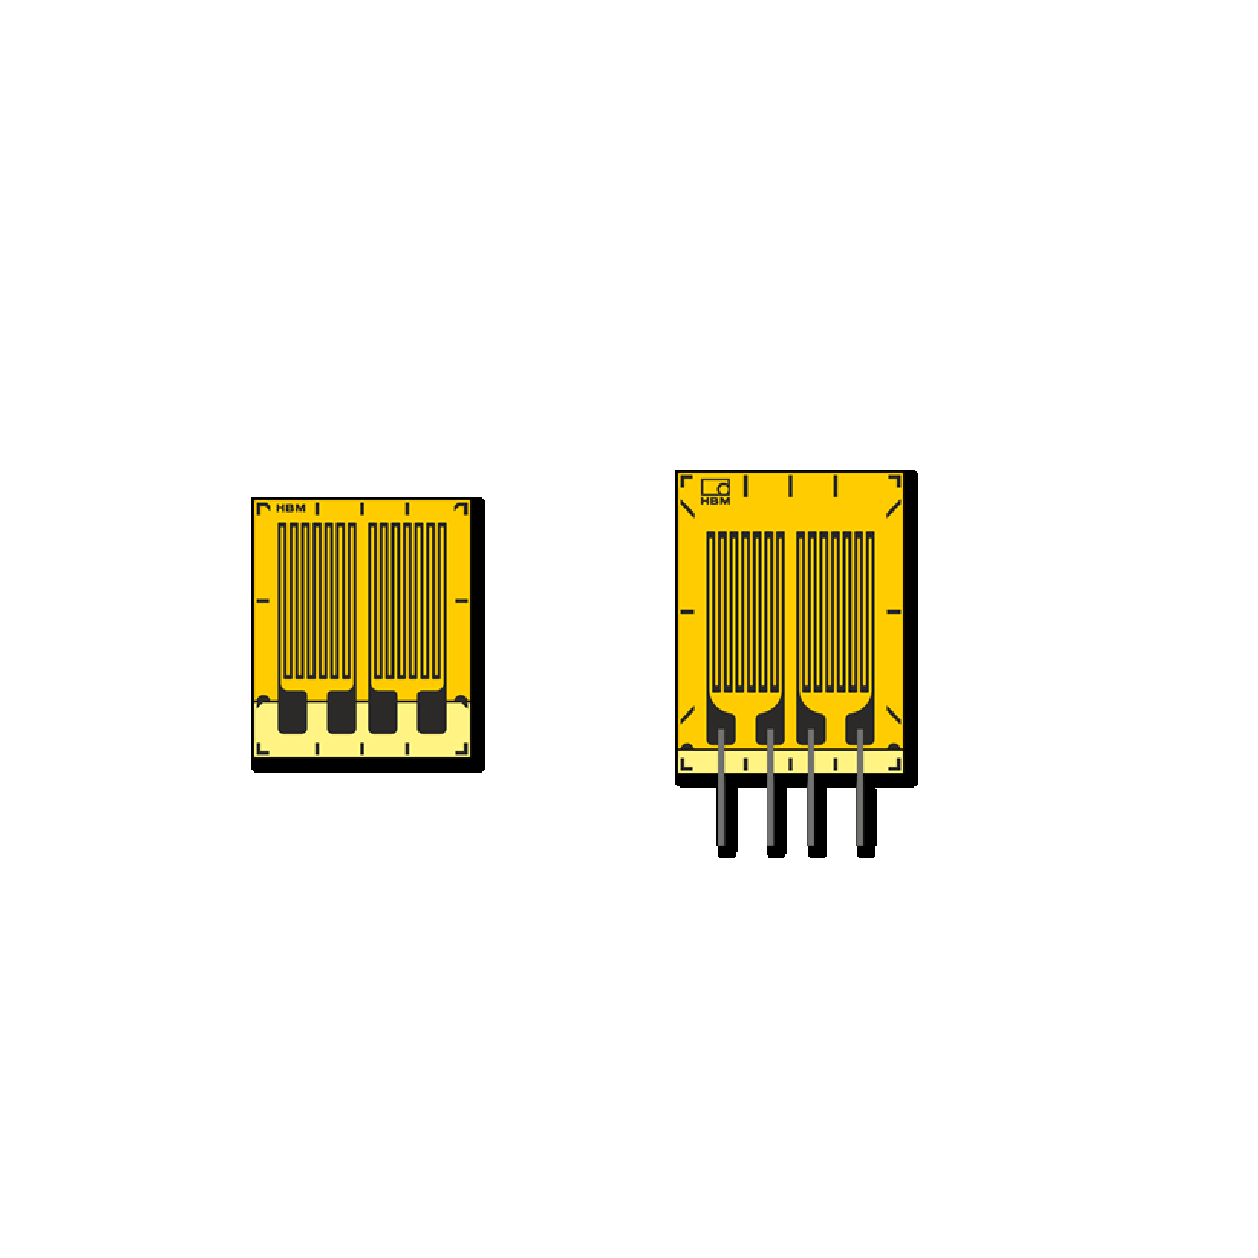
\includegraphics[height=3cm]{bilder/DY.eps}
\end{center}
\caption{DY Doppel-DMS[32]}\label{fig:DY}
\end{figure}


%
\subsection{Elektrische Schaltung der DMS}
Die geringen Widerstandsvariationen eines DMS werden fast ohne 
Ausnahme mit der Wheaststone Br"ucke ermittelt, 
die Abbildung~\ref{fig:w} zeigt die Schaltung: Ub ist eine feste Spannung, 
haupts"achlich eine Gleichspannung, aber es wird auch die Wechselspannung benutzt. 
Dadurch werden unn"otige Thermospannungen entfernt[33].


\begin{figure}[!htb]
\begin{center}
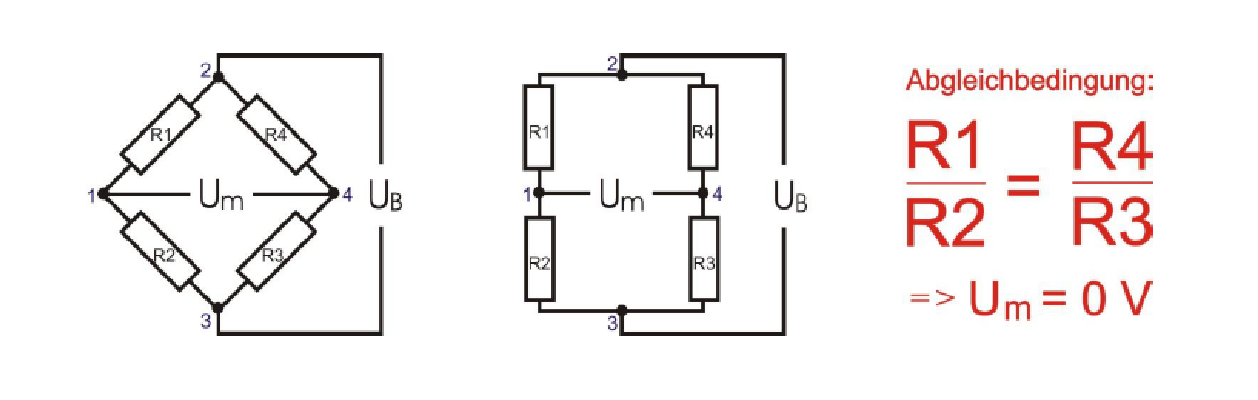
\includegraphics[height=3cm]{bilder/w.eps}
\end{center}
\caption{Wheatestone-Br"ucke mit DMS[33]}\label{fig:w}
\end{figure}





Es ist oft erforderlich, einen negativen Eingang in Arduino zu nehmen. 
 Aber der Arduino nimmt  nur positive Spannungen auf. 
Die unten erkl"arte Methode nimmt die negativen und positiven Werte und 
sendet sie  an Arduino. Die L"osung besteht darin, sowohl den urspr"unglichen 
Eingang als auch einen inversen Eingang zu nehmen und einen mit einem 
Multiplexer auszuw"ahlen. So k"onnen wir den positiven Eingang, wie er ist, 
und den negativen Eingang in umgekehrter Form erhalten. 
Das Signal kann "uber den Ausgang eines Vergleichers bestimmt werden, 
der dem gleichen Eingang wie die Differenzverst"arker ausgesetzt ist.

Die Schaltung besteht aus zwei Differenzverst"arkern. 
Die Schaltung f"ur beide ist genau gleich. 
Aber der angegebene Eingang ist umgekehrt.

(V1-V2 zu einem und V2-V1 zu einem anderen). Man verwendet Operationsverst"arker LM358 ,
 um Differenzverst"arkerteile zu realisieren. 
 Man bekommt zwei Eing"ange, einen umgekehrten und den Original. 
 Wie man dazwischen  w"ahlt, ist im n"achsten Schritt erkl"art. 

Der Vergleich wird benutzt, um das Zeichen des Eingangs 
(negativ oder positiv) zu ermitteln. Eine Komparaturschaltung 
kann mit einem einfachen Operationsverst"arker hergestellt werden. 
Es wird eine positive Feedback gegeben 
(d.h. verbinden Sie die Output mit dem nicht-umkehrenden Anschluss des Operationsverst"arkers) 
mit einem hohen Widerstand. Es wird1Mohm 1K oder 220 Ohm verwendet, 
die auch die Aufgabe erf"ullen sollten. Man schlie"st dem Komparator mit  
zwei Eing"ange (V1 und V2) an. V2 auf nicht invertierende Anschluss und 
V1 auf invertierende Anschluss. Der Komparator gibt den Ausgang Null aus, 
wenn der V2-V1<0 und Vcc wenn der V2-V1>0 ist, und der Ausgang des Komparators wird auch 
als Eingang des Multiplexers (CD4053) verwendet.

Wir haben Jetzt  drei Leitungen :einen tats"achlichen Eingang, 
sein invertiertes Gegenteil und das Vorzeichen des Eingangs. 
Diese drei k"onnen direkt an den Multiplexer verbunden werden und der 
richtige Eingang kann im Code ausgew"ahlt werden (digitalRead() der Vorzeicheneingang) 
oder wenn die Erhaltung eines Pins von Bedeutung ist, 
kann CD4053 mux benutzt werden. Die Schaltug wird in 
die Abbildung~\ref{fig:Dehn}  gezeigt[34].

\begin{figure}[!htb]
\begin{center}
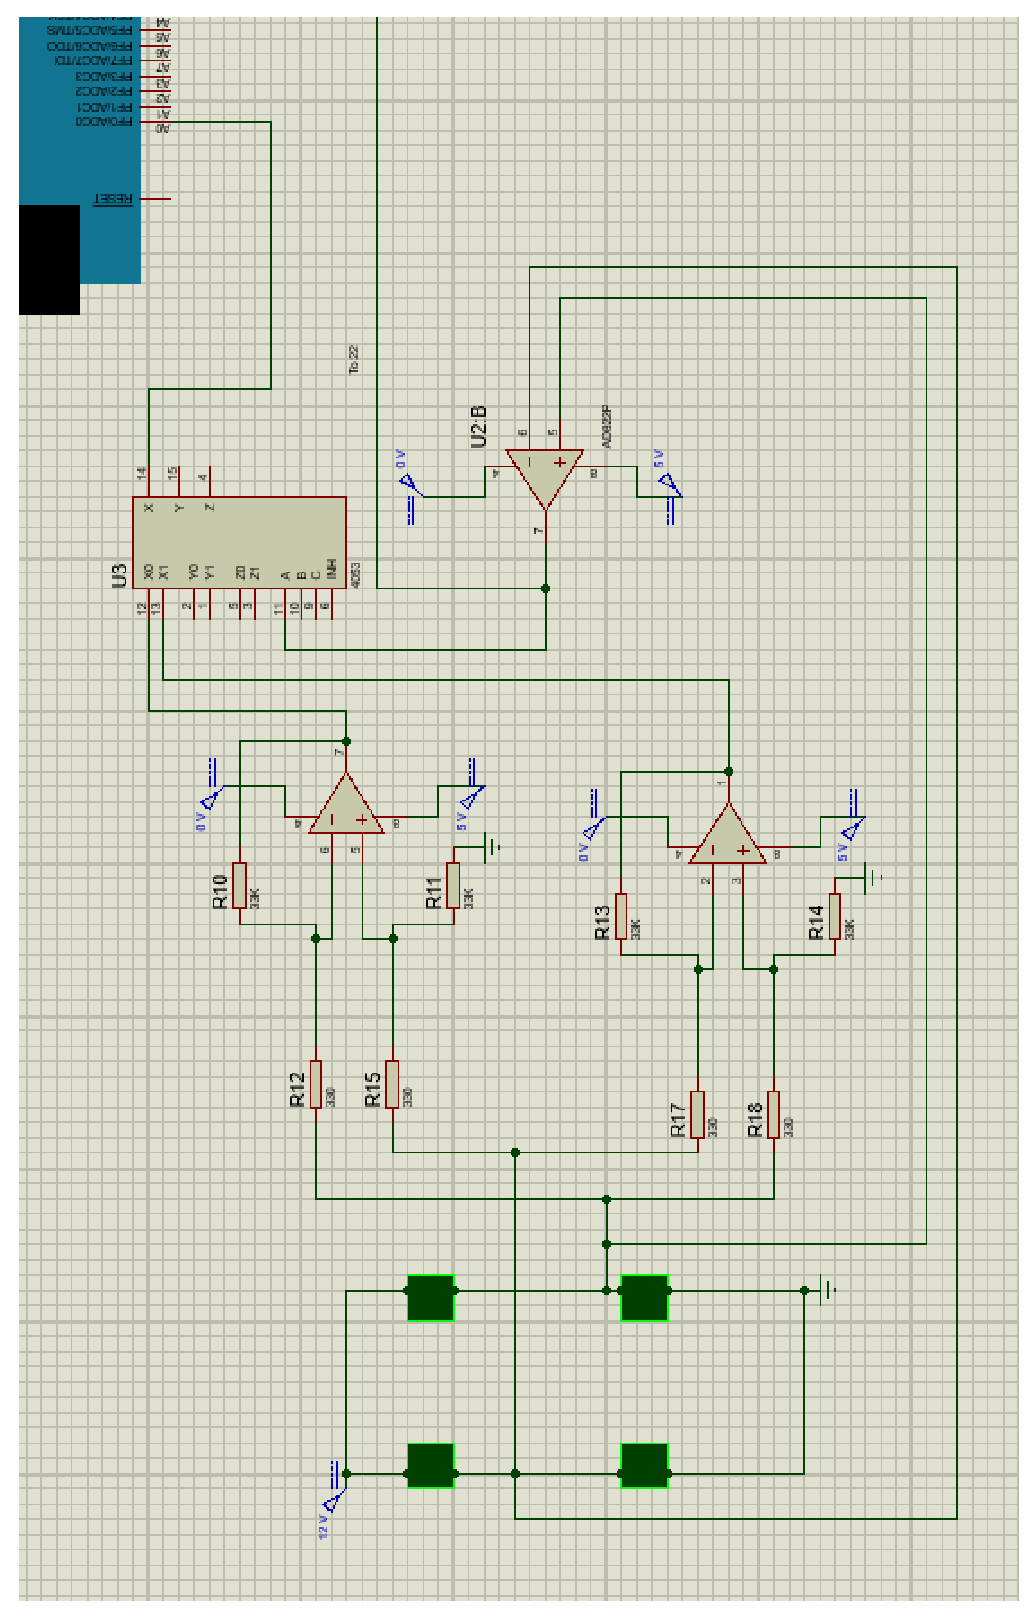
\includegraphics[height=7cm]{bilder/Dehn.eps}
\end{center}
\caption{Schaltung der Dehnmessstreifen}\label{fig:Dehn}
\end{figure}








\subsection{Carnot-Prozess}

Der Carnot-Prozess ist daher ein Modell f"ur zirkul"are Prozesse, 
weil er Energie sehr effizient umsetzt, was er sehr gut kann, 
weil er absolut reversibel funktioniert, mit dem Vorteil, 
dass durch den Carnot-Prozess keine Entropie entsteht. 
Der Nachteil ist, dass es nur in der Theorie funktioniert, 
nicht in der Realit"at. Der Name ist der Carnot-Prozess, 
weil er von dem Franzosen Sadi Carnot erfunden wurde, 
der sich der Effizienzverbesserung von Dampfmaschinen widmete 
und der als sehr inoffiziell bezeichnet wird, 
f"ur den seine wissenschaftlichen Forschungen oft 
wichtiger sind als seine Umgebung[35]. 

Damit dieser zyklische Prozess reversibel ist, 
werden die folgenden Zustands"anderungen ber"ucksichtigt, 
die das Arbeitsmedium st"andig aufsetzt:  \newline
1$\rightarrow$2:  isotherme W"armeaufnahme: Die W"arme"ubertragung erfolgt 
mit unbegrenzten kleinen Temperaturunterschied. 
Die Entropie nimmt zu, aber es findet keine Entropie statt.\newline

2$\rightarrow$3:   Isentrope Expansion: Das Arbeitsmedium-Volumen steigt,
 Druck- und Temperatur sinken.Das l"auft adiabat, das bedeutet ohne W"armestrom,
  ohne Reibung und ohne Energieverlust. \newline
  
3$\rightarrow$4: Isotherme W"armeabgabe: Hier auch erfolgt die W"arme"ubertragung
 mit unbegrenzt kleinen Temperaturunterschieden, so dass nur die Entropie 
 das System verl"asst, die sowieso mit der W"arme zu tun hat, 
 aber es entsteht keine Entropie. \newline
 
4$\rightarrow$1: Isentrope Kompression: Das Arbeitsfluid wird komprimiert,
 dadurch werden Druck und Temperatur erh"oht. 
 Dies geschieht auch adiabasisch und ohne Energieverlust[35]. \newline
 
 Die vier Zustandswechsel haben die Gemeinsamkeit, 
 dass sie nur dann wie dargestellt ablaufen k"onnen, 
 wenn sie unbegrenzt langsam sind und die Maschine unbeschr"ankt gro"s ist. 
 Isotherme Zustands"anderungen treten bei unbegrenzten kleinen 
 Temperaturunterschieden  auf. Damit W"arme verdr"angt werden kann, 
 ist es notwendig, entweder unendlich lange zu warten oder 
 eine unendlich gro"se Fl"ache f"ur die W"arme"ubertragung zur Verf"ugung zu 
 stellen. Und wenn man versucht, isentrope Zustands"anderungen zu 
 erreichen, dann stellt man recht schnell fest, dass man unbegrenzt 
 langsamer arbeiten muss, so dass keine Entropie entsteht[35]. 

 Die Abbildung~\ref{fig:pv} zeigt ,wie man den Carnot-Prozess in einem p,v- Diagramme anzeigen kann.
 \begin{figure}[!htb]
\begin{center}
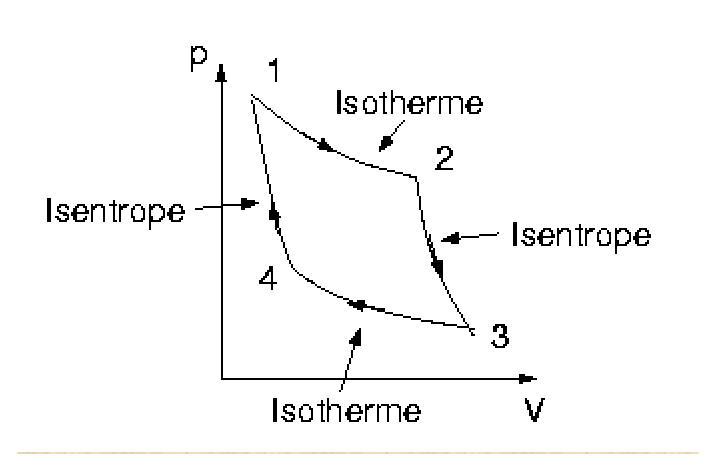
\includegraphics[height=9cm]{bilder/pv.eps}
\end{center}
\caption{PV Diagramm[36]}\label{fig:pv}
\end{figure}





%



 







